\label{chap:problem_formulation}

This chapter discusses in detail the limitations with current display protocol technology that were alluded to in Chapter~\ref{chap:introduction}. From there, it focuses on how these limitations affect adversely IRLED projector technology. Finally, it provides a problem solution.

\section{Display Protocol Limitations}

    Current display technologies, such as HDMI, assume a fixed frame rate display which places a hard limit on frame timing and synchronization.

    % Limitations:
    % Synchronization:
    %   -Implementation and integration-costs $
    %   -System-specific solutions $
    %   -Poor upgradeability $
    In detail, display protocols operate in a best-effort fashion where a buffer swap-initiated transfer of frame data occurs at a static predetermined interval. If a new frame is unavailable to be transmitted at each interval due to any delay, such as processing delay, the previous frame will be retransmitted. This necessarily makes correct synchronization challenging because modern computation systems do not generally provide real-time guarantees due to variability in system operation, including frame generation, CPU scheduling, and Input/Output (I/O) delays. Generally, while these challenges can often be addressed to some degree, they require custom hardware solutions on top of existing display protocols because end-to-end system synchronization is out of the scope of typical display standards which are designed to push relatively low frame rates over single hardware links. These solutions also tend to lack abstraction layers which can greatly hinder upgradeability.

    % Limitations:
    % Display Protocols
    %   -Frame rate limits                 -> image size inversely proportional to speed $
    %   -Static Bandwidth Requirements     -> full image transfer $
    %   -Static frame rates                -> 60Hz, 100Hz, etc. $
    %   -Scalability                       -> single scene generator, projector driver $
    %   Diagrams: Bandwidth diagram -- referenced already $
    Moreover, because of the static nature of the transmission interval (e.g. 100Hz), the frame rate cannot be dynamically controlled or changed after initialization. Instead, these protocols have static bandwidth requirements for a given resolution and frame rate of the form found in Table~\ref{tbl:bandwidth}, which shows that resolution size is inversely proportional to the max speed the display can operate at. Additionally, these protocols only support sending the entire frame at a given interval even if only a small portion of the frame has changed. This is a non-optimal use of bandwidth that does not allow for fine-grained control over the frame rate in cases where a user might wish to dynamically change the frame rate to match the processing rate. In high-speed display scenarios, this inevitably causes dropped frames. This issue is further compounded by the fact that conventional display protocols utilize proprietary drivers and hardware such that frame-drops become effectively silent. Similar to the synchronization solutions discussed above, this tends to lead to upgradeability issues due to systems being tailored for specific display hardware. This contributes to scalability issues as well since changing the display hardware often requires a complete system redesign.

    % Analog Chain:
    %   -RT settling time limitations: -- not included right now
    % Existing diagrams:
    %   Diagrams: scene generator -> Non-uniformity Correction -> Projector
    %   Diagrams: Modeline Overhead diagram

    \begin{table}
        \centering
        \large
        %\begin{small}
        %$$bandwidth = resolution \times bits \times fps$$
        %$bandwidth$ : \quad bandwidth requirements in bits per second. \\
        %$resolution$ : \quad number of pixels including porches. \\
        %$bits$ : \quad \quad \quad \ \ \ bits per pixel. \\
        %$fps$ : \quad \quad \quad \ \ \ frames per second.
        \begin{tabular}{| r l |}
            \hline
            $bandwidth$ & = resolution $\times$ bits $\times$ fps \\ \hline
            $bandwidth$ & : bandwidth requirements in bits per second. \\
            $resolution$ & : number of pixels including porches. \\
            $bits$ & : bits per pixel. \\
            $fps$ & : frames per second. \\
            \hline
        \end{tabular}
        \caption{Bandwidth requirements of a conventional display protocol}
        \label{tbl:bandwidth}
        %\end{small}
    \end{table}

\section{High-speed IRLED Scene Projector Systems}
% How these limitations affect IRSP
% Bottlenecks:
% Hardware limitations:
%   -Physical interconnect bandwidth and latency -> Concurrency/Parallelization $
%   -FPGA/ASIC/IC clock rates                    -> Concurrency/Parallelization $
%   -Analog chain settling times (DAC)           -> Address only the pixels needed $
% Software limitations:
%   -Computational/algorithmic limitations       -> Concurrency/Parallelization $
%   -Poorly optimized software / drivers         -> Do not use $
%   -Fixed frame display                         -> Dynamic frame rate + frame segmentation $
%   -Non-RT scheduling                           -> Realtime schedule / DMA -- not covered below - do i want to cover this?
%   -Lack of control                             -> Use a communication protocol with dynamic control built-in $
%

    Conventional display protocols, which are designed for driving relatively low speed consumer electronics as indicated in Chapter~\ref{chap:display_protocols}, are often utilized in High-speed IRLED IRSP systems. This results in a combination of unnecessary hardware and software limitations being incorporated into systems. This section will discuss these limitations and the general methodology toward alleviating them. Hardware limitations will be discussed first then software limitations.

    \subsection{Hardware Limitations}
        There are several hardware limitations including physical bandwidth, latency, IC clock rates, and analog chain settling times. Often the hardware that data is transferred over within these systems has inherent bandwidth and latency limitations that cannot be overcome either due to the nature of physics or simply because faster hardware is not available. One solution toward working around bandwidth issues is to introduce more parallel links into a system. A similar issue arises with respect to the clock rates of components within a system, such as, projector driver firmware, and scene generator. Ideally, these components will operate as fast as possible, but the reality is that the large fan out of I/O signaling needed by arrays can cause critical timing closure issues within FPGA based firmware implementations. Careful routing and planning can help alleviate these issue as well as parallelizing projector drivers such that less signals are driven from a single FPGA component. The speed of the analog chain in these systems is dictated by the digital to analog converter (DAC) and amplifier settling times which can be alleviated by increasing the number of converters utilized within a system if supported by an array. This could increase write speeds by allowing more DACs and amplifiers to drive smaller portions of an array in parallel. All the solutions discussed in this section involve increasing the number of parallelized components operating within a system in order to reduce physical bottlenecks.

    \subsection{Software Limitations}
        In terms of software, computational and algorithm limitations exist in the generation of scenery for display, and in correcting for pixel and array imperfections as well as in putting data into the correct format to be understood by the driving firmware of a projector. Rendering of individual frames of a scene can be particularly computationally expensive. This can be further complicated by poorly optimized software drivers or algorithms. Additionally, in these systems, tight control over timing is important because frame drops are not tolerable. Meaning that fixed rate display technology is a hinderance in terms of user level control. One solution is to utilize technology that allows for dynamic frame rates and frame segmentation, which, requires protocols with dynamic control built in.


\section{Problem Statement}
    IRSP systems need to be capable of operating at high speeds with large resolutions to meet the needs of the sensor testing community. Typically, this can be on the order of 2048 by 2048 pixels with up to 1KHz frame rates with subframe latency. Necessarily, these goals represent a challenging problem to overcome when utilizing typical display technology which is further hindered due to the limitations discussed above. Given these constraints, the question what an appropriate solution is to address the aforementioned issues arises. The central question we could ask ourselves is, how to architect a generalizable, dynamic, and scalable IRSP system capable of High-performance operation, sub-frame latency, dynamic frame rates, and dynamic bandwidth utilization?

\section{Problem Solution}
    Within the current display protocol technology, any effort to address the aforementioned issues requires system developers to have complete control over an entire end-to-end system for a given solution to operate correctly. This means that in practice customized hardware and software that deviates from standard display protocol behavior is required. Any solution that lacks these requirements would fail to completely address operational issues with performance.

    In short, to truly address issues within the conventional display protocol would require creating a new system specific protocol tied to specific custom hardware. Additionally, with this type of solution, it is still not possible to achieve true sub-frame latencies due to the nature of display protocols requiring transmission of entire frames of data at a given interval or frame rate. In practice, IR projector systems are often forced to introduce intermediate buffers within a system in order to ensure correct operation.

    I believe that any effort to address the aforementioned issues and answer our problem statement requires developing a hardware agnostic alternative display protocol designed specifically for high-speed low-latency frame transmission. This would allow for the protocol be retrofitted within existing systems as well as allow for upgradeability, and support for future hardware. In order, to achieve sub-frame latencies, this protocol would need to support transmission of sub-frames of data, i.e. transmission of partial frames. Allowing for partial frame transmission enables a host of other desirable features, such as, the ability to control bandwidth utilization and the ability to incorporate dynamic frame rates. A good method of supporting partial frame transfer is to utilize headered packets of data to provide a context for what the data represents and where to draw said data on a display. This method of transferring display data is called a packetized display protocol (PDP).

    As discussed briefly in the Chapter~\ref{chap:introduction}, this PDP architecture eschews with assumptions found in conventional display technologies to provide a robust feature-set. In contrast to a normal display protocols, the proposed architecture, is designed to utilize a dynamic source driven refresh rate through the coordination of both source (scene generator) and sink (display). In this architecture, frames are segmented into pieces and sent to the display based upon how often these segments need to update. An example of this is shown in Figure~\ref{fig:variable_display} where different regions of the display operate at different frame rates. By utilizing dynamic frame rate control at sub-frame resolutions, substantial bandwidth reductions can occur. This will be discussed in further detail in Chapter~\ref{chap:pdp_protocol}.

    \begin{figure}
        \centering
        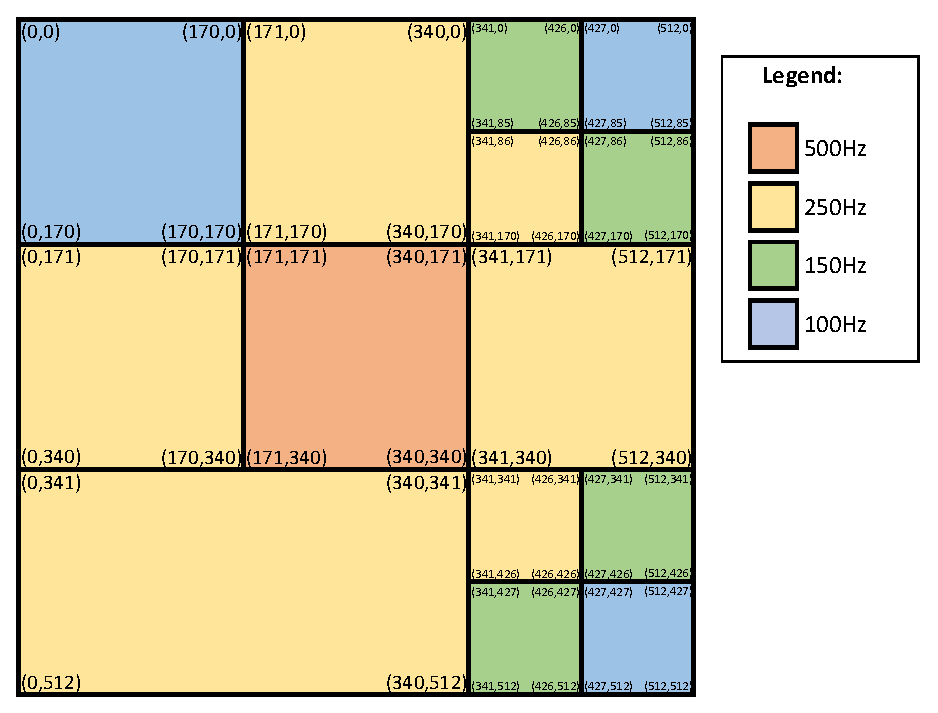
\includegraphics[width=1.0\textwidth]{fig/variable_display.pdf}
        \caption{Dynamic frame rate display with multiple regions updating at different frame rates}
        \label{fig:variable_display}
    \end{figure}

    The underlying PDP itself is designed to allow for fine-grained control over when and what data is transmitted as well as to incorporate mechanisms to synchronize displays. Furthermore, the protocol architecture is abstracted in such a way that the physical interconnect layers are transparent in order to enable it to be capable of operating over a wide-spectrum of hardware as well as to allow the protocol to be extended and used within future hardware. For system upgradeability, this offers a risk reduction because it allows for a simpler migration path as new hardware becomes available. For example, a hardware system implementing this protocol could switch or upgrade physical components and still utilize the same protocol within the software stack given an appropriately compatible physical layer. To further facilitate this, a packetized protocol structure capable of transmitting pixel data in a generalized way has been chosen. These details will be discussed in Chapters~\ref{chap:pdp_protocol} and~\ref{chap:machine_model}.

    The remainder of this work is devoted to discussing the details of the environment in which the PDP is designed to operate, the protocol itself, and its implementation. The following chapter provides an overview of system operation.
